\section{بیان مسئله و مجموعه داده}
\label{sec:dataset}

در این بخش، ابتدا مفاهیم پایه‌ای مرتبط با باتری لیتیوم-یون، ظرفیت و عمر چرخه‌ای معرفی می‌شود و سپس مسئله بیان شده و مجموعه داده مورد استفاده توضیح داده می‌شود.


\subsection{باتری لیتیوم-یون}

باتری‌های لیتیوم-یون گروهی از باتری‌های قابل شارژ به شمار می‌روند. این باتری‌ها از سه بخش الکترود مثبت، الکترود منفی و الکترولیت تشکیل شده‌اند. معمولاً الکترود منفی از کربن و الکترود مثبت از اکسید فلزی ساخته می‌شود و الکترولیت نیز از نمک لیتیوم در یک حلال آلی تشکیل شده است. هنگام دشارژ، یون‌های لیتیوم از الکترود منفی به‌سمت الکترود مثبت حرکت می‌کنند و در هنگام شارژ، جهت حرکت آن‌ها معکوس می‌شود.

عملکرد باتری‌های لیتیوم-یون بر پایه چرخه‌های شارژ و دشارژ است. در فرایند شارژ\LTRfootnote{Charging}، انرژی الکتریکی به باتری وارد شده و ذخیره می‌شود. در مقابل، طی فرایند دشارژ\LTRfootnote{Discharging}، انرژی ذخیره‌شده در اختیار مصرف‌کننده قرار می‌گیرد. مجموع این دو فرایند، یک چرخه شارژ و دشارژ را تشکیل می‌دهد.

\subsection{ظرفیت، عمر چرخه‌ای و پایان عمر}

یکی از مهم‌ترین ویژگی‌های باتری، ظرفیت آن است؛ این کمیت مقدار بار الکتریکی‌ای را نشان می‌دهد که باتری می‌تواند ذخیره و در اختیار مصرف‌کننده قرار دهد و بر حسب آمپرساعت (\lr{Ah}) اندازه‌گیری می‌شود. با تکرار چرخه‌ها و استفاده مداوم، فرایندهای شیمیایی و فیزیکی مختلفی در ساختار باتری رخ می‌دهد که موجب کاهش تدریجی ظرفیت قابل استفاده باتری می‌شوند؛ این فرایند تخریب باتری نام دارد.

با ادامه این فرایند، ظرفیت باتری به‌اندازه‌ای کاهش می‌یابد که عملکرد آن دیگر برای کاربرد موردنظر قابل قبول نخواهد بود. این وضعیت پایان عمر باتری\LTRfootnote{End of Life (EOL)} نامیده می‌شود. در بسیاری از پژوهش‌های مربوط به باتری‌های لیتیوم-یون، رسیدن ظرفیت به ۸۰ درصد ظرفیت اولیه باتری به‌عنوان معیار پایان عمر در نظر گرفته می‌شود. تعداد چرخه‌هایی که باتری پیش از رسیدن به این آستانه طی می‌کند، عمر چرخه‌ای\LTRfootnote{Cycle Life} نام دارد و یکی از شاخص‌های مهم برای ارزیابی دوام و طول عمر باتری است.
\subsection{بیان مسئله}

بسیاری از پژوهشگران مدل‌های فیزیکی و نیمه‌تجربی مختلفی ارائه کرده‌اند که سازوکارهای گوناگون تخریب باتری را در نظر می‌گیرند؛ از جمله رشد لایه مرزی جامد-الکترولیت\LTRfootnote{Solid Electrolyte Interphase (SEI)}، رسوب فلز لیتیوم\LTRfootnote{Lithium Plating}، کاهش مواد فعال الکترود و افزایش امپدانس باتری. در سامانه‌های مدیریت باتری\LTRfootnote{Battery Management System (BMS)}، پیش‌بینی عمر مفید باقی‌مانده\LTRfootnote{Remaining Useful Life (RUL)} نیز که در پژوهش‌ها‌ی پیشین بررسی شده است، اغلب بر مدل‌های مبتنی بر سازوکارهای فیزیکی و نیمه‌تجربی برای تخمین وضعیت باتری تکیه دارد.

اگرچه مدل‌های طراحی‌شده بر اساس شیمی باتری یا سازوکارهای تخریب آن در پیش‌بینی عملکرد موفقیت‌هایی داشته‌اند، توسعه مدل‌هایی که بتوانند رفتار سلول‌های کامل باتری را در شرایط کاری واقعی (برای مثال، شارژ سریع) توصیف کنند، همچنان چالش‌برانگیز است. دلیل این دشواری، وجود سازوکارهای متعدد تخریب و همچنین تأثیر متقابل آن‌ها با ناهمگونی‌های حرارتی و مکانیکی درون سلول باتری است\cite{severson2019}.

در این روش، اطلاعات ثبت‌شده در چرخه‌های مختلف باتری، شامل ولتاژ\LTRfootnote{Voltage}، دما\LTRfootnote{Temperature} و ظرفیت دشارژ\LTRfootnote{Discharge Capacity}، به‌عنوان ورودی یک شبکه عصبی کانولوشنی (CNN) به کار می‌روند. شبکه با یادگیری الگوهای موجود در داده‌های عملکردی باتری، رابطه میان ویژگی‌های اندازه‌گیری‌شده و مقدار RUL را استخراج می‌کند. هدف نهایی آن است که مدل بتواند بر اساس اطلاعات یک چرخه مشخص، مقدار RUL باتری را تخمین بزند و بدین ترتیب امکان ارزیابی وضعیت تخریب و پیش‌بینی زمان تقریبی پایان عمر مفید باتری فراهم شود.

\subsection{مجموعه داده}

در این پروژه، از مجموعه‌داده‌ای شامل ۴۰ سلول باتری لیتیوم-یون استفاده شده است. مجموعه‌داده کامل شامل ۱۲۴ سلول است که به‌منظور تسهیل اجرای پروژه، زیرمجموعه‌ای شامل ۴۰ سلول از آن انتخاب شده است\cite{mathworks}. این باتری‌ها دارای ظرفیت اسمی ۱٫۱ آمپرساعت و ولتاژ اسمی ۳٫۳ ولت هستند. پایان عمر هر باتری نیز زمانی در نظر گرفته شده است که ظرفیت آن به ۸۰ درصد ظرفیت اسمی اولیه برسد.

باتری‌های موجود در مجموعه داده با سیاست‌های شارژ متفاوتی آزمایش شده‌اند و مدت‌زمان و شرایط فرایند شارژ در آن‌ها یکسان نیست. این تفاوت‌ها می‌توانند باعث تغییراتی در داده‌های شارژ شوند که لزوماً ناشی از تخریب باتری نیستند. در مقابل، شرایط دشارژ همه باتری‌ها یکسان است و این فرایند در محدوده ولتاژ ۳٫۶ تا ۲ ولت انجام می‌شود. بنابراین، به‌منظور کاهش تأثیر تفاوت شرایط آزمایش و فراهم‌کردن امکان مقایسه بهتر باتری‌ها، ویژگی‌ها و ورودی‌های مدل از اطلاعات فرایند دشارژ در این محدوده ولتاژ استخراج شده‌اند.

\begin{figure}[!htbp]
\centering
\begin{minipage}{0.48\textwidth}
\centering
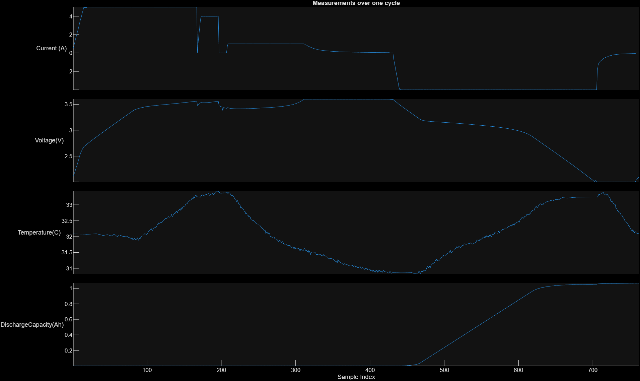
\includegraphics[width=\linewidth]{img/cycle-full.png}
\par\smallskip
\textbf{(الف)} چرخه کامل شارژ و دشارژ
\end{minipage}\hfill
\begin{minipage}{0.48\textwidth}
\centering
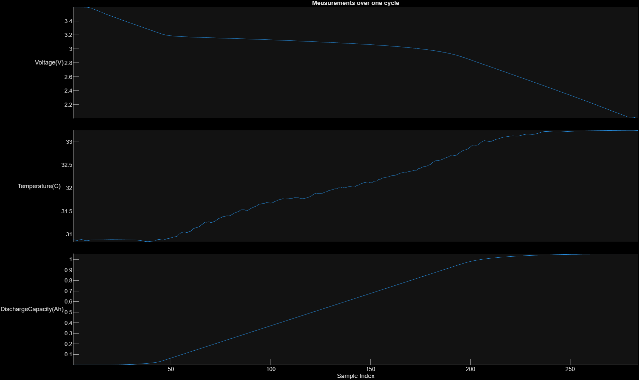
\includegraphics[width=\linewidth]{img/cycle-discharge.png}
\par\smallskip
\textbf{(ب)} مرحله دشارژ
\end{minipage}
\caption{مقایسه داده‌های ثبت‌شده در یک چرخه کامل(شامل شارژ و دشارژ) و داده‌های مربط به مرحله دشارژ؛ در هر دو نمودار، تغییرات ولتاژ، دما و ظرفیت دشارژ نمایش داده شده است.}
\label{fig:cycle}
\end{figure}

برای هر باتری و در هر چرخه شارژ و دشارژ، اطلاعات زیر جمع‌آوری و ذخیره شده‌اند:
\begin{itemize}
\item جریان الکتریکی
\item ولتاژ
\item دما
\item ظرفیت باتری
\item ظرفیت تفاضلی دشارژ
\end{itemize}

از میان این کمیت‌ها، سه ویژگی ولتاژ، دما و ظرفیت دشارژ به‌عنوان ورودی شبکه عصبی انتخاب شده‌اند (بخش~\ref{sec:preprocessing}). تفاوت میان داده‌های یک چرخه کامل و داده‌های مرحله دشارژ در شکل~\ref{fig:cycle} نشان داده شده است. همان‌طور که در شکل دیده می‌شود، در این پروژه داده‌های مرحله دشارژ مبنای استخراج ویژگی‌ها قرار می‌گیرند.
